\chapter{Background}\label{ch:background}

\section{Continuous-time Markov Chains}
A \emph{stochastic process} is a parameterized collection of random variables $\{X_t\}_{t\in T}$ defined on some probability space $(\Omega, \mathcal{F}, P)$ and takes values in complete metric space $(\mathcal{S}, r)$.
\marginpar{See \citet{feller} for stoch.\ processes in general.}
In most contexts the index set $T$ models \emph{time}.
In a discrete setting $T=\mathbb{N}$, while $T=[0,\infty)$ in the continuous setting, which we consider in this thesis.
We observe the values $X(t, \omega)$ for some fixed, but unknown $\omega\in\Omega$.
The information of the process up to time $t$ is given by the $\sigma$-algebra $\mathcal{F}_t\subset\mathcal{F}$.
The increasing family of sigma algebras, i.e.\ $\mathcal{F}_s\subseteq\mathcal{F}_t$ for $s\leq t$ is called a \emph{filtration}.

More specifically, we study with models having \acf{CTMC} semantics --- a type of \emph{Markov process}.
Such processes satisfy the \emph{Markov property}:
For all Borel-measurable functions $f$
\begin{equation}\label{eq:markov_prop}
    \E{f(X_{t+s})\mid \mathcal{F}_t} = \E{f(X_{t+s})\mid X(t)}\,.
\end{equation}
Intuitively, this property expresses that the future of the process depends only on the latest condition, i.e.\ $X_{t}$ and not earlier conditions ($\mathcal{F}_t$).
A \ac{CTMC} is a Markov process, that takes discrete values $\mathcal{S}=\{s_0, s_1,\dots\}$ over continuous time $T=[0,\infty)$.\marginpar{The time-discrete analogue is the \ac{DTMC}\@.}
If further
\begin{equation}\label{time_homo}
    \Pr\left(X_t=s_1\mid X_0 = s_0\right)
    =\Pr\left(X_{t+h}=s_1\mid X_h=s_0\right)
\end{equation}
for all $t,h\geq 0$ and $s_0, s_1\in\mathcal{S}$ the chain is \emph{time-homogenous}:
The absolute time point is irrelevant, and the dynamics do not change if we shift in time.
In this thesis we are only interested in tim-homogenous \acp{CTMC}, but most techniques
developed should carry over.
We define \emph{transition probabilities}
\begin{equation}
    p_{ij}(h) = \Pr(X_h = s_j\mid X_0=s_i)\,.
\end{equation}
Accordingly, the \emph{transition matrix} is given by $P(h)_{ij} = p_{ij}(h)$ for all indices $i$ and $j$.
The Chapman-Kolmogorov equation
\begin{equation}\label{eq:chapman_kolm}
    P(s+t) = P(s)P(t)
\end{equation}
follows directly from the law of total probability and the Markov property \eqref{eq:markov_prop}.
\eqref{eq:chapman_kolm} directly tells us that the transition probabilities
from a semigroup.
Studying Markov processes from this direction is a popular approach \parencite{ethier2009markov}.

The standard method of specifying a Markov process, and \acp{CTMC} in particular, is
is the \emph{generator}.
In general, this is an operator $A$ on some class of functions and
\begin{equation}\label{eq:generator}
    \E{f(X_{t+h}) - f(X_t)\mid \mathcal{F}_t}
    =
    Af(X_t)h + o(h)\,,
\end{equation}
where $\mathcal{F}_t$ is the filtration up to time $t$.
This equation can be interpreted as the requirement, that
\[f(X_t) - f(X_0) - \int_0^t Af(x_s)\,ds\] is a martingale \parencite[see][p.~5]{kurtz1981approximation}.
We will use this in \autoref{ch:MFPT} to derive bounds on \aclp{MFPT}\@.

In \acp{CTMC} the generator is defined by giving the \emph{intensities} or \emph{rates}
of transitions.
Such a rate $q_{ij} > 0$ between state $s_i$ and $s_j$ implies\marginpar{This is congruent with \eqref{eq:generator} under application the Markov property.}
\begin{equation}
    \Pr(X_{h} = s_j\mid X_0=s_i) = q_{ij}h + o(h)\,.
\end{equation}
%The $Q$-matrix characterizes the distributional change in the infinitesimal time interval:
Due to the discrete nature, the generator is a matrix, usually called the $Q$-matrix,
\begin{equation}
    Q = \lim_{h\downarrow 0}\frac{1}{h}\left(P(h) - I\right)\,.
\end{equation}
As such the change of the state probability distribution over time is fully characterized by the \emph{Kolmogorov forward equation}
\begin{equation}\label{eq:kolm_forw}
    \frac{d}{dt}P(t) = P(t)Q\,.
\end{equation}
Analogously, the \emph{Kolmogorov backward equation} is
\begin{equation}\label{eq:kolm_back}
    \frac{d}{dt}P(t) = QP(t)^{\T}\,.
\end{equation}
Distributions in the context of Markov chains are typically in row-vector form
\[
\pi(t)\coloneqq(\pi(x_1, t), \pi(x_2, t), \dots)\,,
\]
where we define
\[
\pi(x_i, t)\coloneqq \Pr(X_t=x_i), \quad\forall x_i\in\mathcal{S}, \forall{t\geq 0}\,.
\]
Often, \eqref{eq:kolm_forw} and \eqref{eq:kolm_back} are used in the context of an
distributions.
In this case it makes more sense to right-multiply the unit vector to these equations such
that
\begin{equation}\label{eq:kolm_forw_d}
    \frac{d}{dt}\pi(t) = \pi(t)Q
\end{equation}
and
\begin{equation}\label{eq:kolm_back_d}
    \frac{d}{dt}\pi(t) = Q\pi(t)^{\T}\,.
\end{equation}
Given some initial distribution
\[
\pi_0 \coloneqq \pi(0)\,,
\]
the distribution $\pi(t)$ is given by give simple \acp{IVP} of \eqref{eq:kolm_forw_d}.

\subsection{Computing Transient Distributions}
\citet{stewart1994introduction} provides a comprehensive overview of solution methods.
Here, we only provide a basic overview and intuition relevant for the rest of this thesis.
\begin{description}
    \item[Matrix exponential]
        The transition probability matrix $P(t)$ is the solution of \eqref{eq:kolm_forw}
        \[
            P(t)=\exp(Qt)\,,
        \]
        where the matrix exponential for a square matrix $M$
        \[
        \exp({M})\coloneqq\sum_{k=0}^{\infty}\frac{1}{k!}M^k\,.
    \]
        Due to the factor ${h^k}/{k!}$, the sum of the matrix exponential
        can be truncated to get an estimate
        of high quality. In practice, this method is unsuited to many problems, because
        the factor $Q^k$ becomes incurs a prohibitive cost, especially if the state space
        is large.
    \item[Numerical integration]
        The Kolmogorov equations \eqref{eq:kolm_forw}, \eqref{eq:kolm_back}
        provide us with an \ac{IVP} that can be solved
        numerically.\graffito{The matrix exponential is the analytical solution.}
        This method scales much better than the matrix exponential method,
        especially if the whole time-series is of interest. If an initial distribution
        $\pi_0$ is fixed, the \ac{ODE} simplify further, such that we only have one equation
        per state.
        The drawback to this method is the error inherent to numerical
        integration schemes.
    \item[Uniformization]\label{item:uniformization}
        Uniformization is an elegant algorithm to compute transient solutions.
        Here, the \ac{CTMC} is transformed into a \ac{DTMC}\@.
        Using a uniformization rate \[\lambda_0\geq\max_{i}\lvert q_{ii}\rvert\]
        the transition probabilities of the \ac{DTMC} become
        \[
        P_{ij} =
        \begin{cases}
            Q_{ij} / \lambda_0\,, &\text{if } i\neq j\\
            1 - \sum_k Q_{ik} / \lambda_0\,, &\text{otherwise}
        \end{cases}\,.
    \]
        The transient distribution at $t$ can be obtained, by weighting the $k$-step
        probabilities of the \ac{DTMC} by a Poisson distribution with rate
        $\lambda_0 t$:
        \[
        \pi(t) =
        \sum_{k=0}^{\infty}\pi_0P^k\frac{(\lambda_0 t)^k}{k!} \exp{(\lambda_0 t)}\,.
    \]
        Truncation of this series clearly gives an underapproximation.
    \item[Monte Carlo simulation]
        A simple way is estimation using Monte Carlo methods. This entails stochastic
        simulation of many trajectories of the \ac{CTMC}\@\@. Generating a trajectory is
        straightforward: Given that the process is in a particular state $s_i$
        the a transition has to be sampled along with the residence time in state
        $s_i$. The naive approach is to sample an exponential random variable for
        each $q_{ij}$ and choose the one firing first.
        This algorithm can be improved by sampling a reaction directly and
        sampling the residence time separately. This algorithm will be shown later
        in the context of \acp{MPM}\@.\turnto{alg:ssa}
\end{description}
% \begin{itemize}
%    \item Properties (non-explosivity, ergodicity, reversibility, irreducibility etc.)
% \end{itemize}

\section{Markovian Population Models}
An \acf{MPM}
among agents of $n_S$ distinct types in a well-stirred system.
Other names for this model class are \acf{pCTMC}, \acf{CRN}, and \acf{SRN}\@.
The system is given by a continuous-time stochastic process $\{X_t\}_{t\geq 0}$.
It models only the number of agents according to their type.
Therefore the process takes $n_S$-dimensional vectors of natural numbers as values, i.e.\ the
state-space is $\mathcal{S}\subseteq\mathbb{N}^{n_S}$.
\marginpar{
    ``The secret to modelling is not being perfect.''
    \begin{flushright}
        \emph{--- Karl Lagerfeld}
\end{flushright}
}
By only considering the number of agents, we are neglecting factors such as spatial variations
in agent density or other factors influencing interactions.
The assumption of all agents being equally distributed in space is called the \emph{well-stirredness}
assumptions.

These assumptions bring with them, the convenience of considering populations as a whole.
The single agent is of no importance to the dynamics of the process.
Just the overall size of each population determines the stochastic evolution of the process.
Another consequence of this assumption is the limiting behaviour under this assumption.
If all populations are proportionally scaled to infinity, their concentrations can be accurately described by deterministic \acp{ODE}\@.
\marginpar{Other assumptions, such as exponentially distributed firing times are discussed below.}
In fact, this is the most widely used paradigm to analyze this kind of reaction networks.
However this methodology may by widely inaccurate.
Consider, for example, an epidemic process.
Typically individuals are not well-stirred in a societal context and the influence of specific
contact structures is crucial to the process' dynamics \parencite{grossmann2020importance,grossmann2021heterogeneity}.
Furthermore such a process typically exhibits discrete stochastic effects, such as the epidemic dying out.
While the latter effect is retained in an \ac{MPM}, the former is already lost.
Therefore, a great deal of care has to be taken by the modeller which kinds of abstractions are appropriate for the chosen abstraction.

Interactions between agents are expressed as \emph{reactions}.
These reactions have associated
gains and losses of agents, given by non-negative integer vectors
${v}_j^{-}$ and ${v}_j^{+}$ for reaction $j$, respectively. The overall change by a reaction is given by the vector $v_j = v_j^+ - v_j^-$.
A reaction between agents of types $S_1,\dots, S_{n_S}$ is specified in the following form:
\begin{equation}\label{eq:reaction}
    \sum_{\ell=1}^{n_S} v_{j\ell}^{-} S_\ell
    \xrightarrow{\alpha_j( x)}
    \sum_{\ell=1}^{n_S} v_{j\ell}^{+} S_\ell\,.
\end{equation}
The propensity function $\alpha_j$ gives the rate of the exponentially distributed firing
time of the reaction as a function of the current system state $x\in \mathcal{S}$.
Thus, for reaction $j$ we have the intensity
\begin{equation}\label{eq:firing}
    \Pr\left(X_{t+h}=x+v_j\mid X_{t}=x\right)
    =
    \alpha_j(x) + o(h t)\,.
\end{equation}


In most physical models, \emph{mass-action} propensities are most common.
These model combinatorial nature of well-mixed molecules moving randombly through space:
In a reaction
\[ A + B \xrightarrow{c x^{(A)} x^{(B)}} C \]
two molecules hit eachother with a probability, proportional to the product of their counts
\[ c X^{(A)}_t X^{(B)}_t\,. \]
In general such rates are given by the product of the number
of reactant combinations in $x$ and a
\emph{rate constant} $c_j$, i.e.
\begin{equation}\label{eq:stoch_mass_action}
    \alpha_j({x})\coloneqq c_j\prod_{\ell=1}^{n_S}\binom{x^{(S_{\ell})}}{v_{j\ell}^{-}}\,.
\end{equation}
In this case, we give the rate constant in \eqref{eq:reaction} instead of the function $\alpha_j$.
We use the superscript notation\marginpar{This notation avoids conflicts, when we use the subscript for time or as an index.} $x^{(A)}$ to denote the index corresponding to species $A$
in some vector of length $n_S$.

According to \eqref{eq:firing} the stochastic
process $\{{{X}}_t\}_{t\geq 0}$ describing the evolution of the population
sizes over time $t$ is a \acf{CTMC}\@.
The infinitesimal  generator matrix $Q$ has the entries
\begin{equation}\label{eq:cme_generator}
    Q_{ x,  y} = \begin{cases}
        \sum_{j: x+ v_j = y}\alpha_j( x)\,,&\text{if}\; x\neq
         y,\\[1ex]
        -\sum_{j=1}^{n_R} \alpha_j( x)\,, &\text{otherwise.}
    \end{cases}
\end{equation}
Note that in addition mild regularity assumptions
are   necessary for the existence of a unique \ac{CTMC} $X$, such as non-explosiveness \parencite{anderson2012continuous}.
These assumptions  are  typically
valid for realistic reaction networks.
The probability distribution over time is given by an
initial value problem.
Given an initial state $x_0$, the probabilities%\graffito{We assume an enumeration of all states in  $\mathcal{S}$ with a unique index for each state.}
\begin{equation}\label{eq:forw_prob}
    \pi(x_i, t)\coloneqq\Pr(X_t=x_i\mid X_0=x_0),\quad t\geq 0,\quad x\in\mathcal{S}
\end{equation}
evolve according to the Kolmogorov forward equation
\begin{equation}\label{eq:forward}
\frac{d}{dt}\pi(t) = \pi(t) Q\,,
\end{equation}
where $\pi(t)$ is an arbitrary vectorization \[(\pi(x_1,t), \pi(x_2,t),\dots,\pi(x_{|\mathcal{S}|},t))\] of the state probabilities.
Often \eqref{eq:forward} is given for a single state.
In this form --~due to its usage in quantitative biology~-- it is commonly referred to
as the \emph{\acf{CME}}
\begin{equation}\label{eq:cme}
    \frac{d\pi}{d t} ( x,t) =
    \sum_{j=1}^{n_R}\left(
        \alpha_j( x- v_j)\pi( x- v_j,t) - \alpha_j( x)\pi( x,t)
    \right)\,.
\end{equation}



\begin{example}
Consider the following simple \ac{MPM} with non-linear propensities as an example.
\begin{model}[Dimerization]\label{model:dim}
  We first examine a simple dimerization model on an unbounded state-space with
  reactions
\[
    \varnothing\xrightarrow{\lambda}M,\quad 2M\xrightarrow{\delta}D
\]
  and initial condition $X_0^{(M)}=X_0^{(D)}=0$.
\end{model}
The semantics is given by a \ac{CTMC} $\vec{X}_t=(X_t^{(M)}, X_t^{(D)})^{\T}$, where $(S_1, S_2)=(M,D)$.
The reaction propensities according to~\eqref{eq:stoch_mass_action} are
\[
    \alpha_1(\vec{x})=\lambda
    \quad
    \text{and}
\quad
    \alpha_2(\vec{x})=\delta\, x^{(M)} (x^{(M)} - 1)/2\,.
\]
The change vectors for the first reaction are
\[
    v_1^-={(0,0)}^{\T}\quad\text{and}\quad v_1^+={(1,0)}^{\T}\,.
\]
For the second reaction the change vectors are
\[
    v_2^-={(2,0)}^{\T}\quad \text{and}\quad v_2^{+}={(0,1)}^{\T}\,.
\]
Consequently, $v_1={(1,0)}^{\T}$ and $v_2={(-2, 1)}^{\T}$.

The generator matrix
\[
    Q = \begin{bmatrix}
        -\lambda & \lambda & 0 & & & &\cdots \\
        0 & -\lambda & \lambda & 0 & && \cdots\\
        2 \delta & 0& -(\lambda + 2\delta) & \lambda & 0 && \cdots \\
        0 & 6\delta & 0 & -(\lambda + 6\delta) & \lambda &0&\cdots \\
        \vdots & \vdots & \vdots & \vdots & \vdots & \vdots&\ddots
    \end{bmatrix}\,.
\]
Often it is a good idea to visualize the state-space and transitions as a graph.
This graph is constructed by interpreting the $Q$-matrix as an adjacency matrix for some subset of states.
\begin{figure}[h!]
    \centering
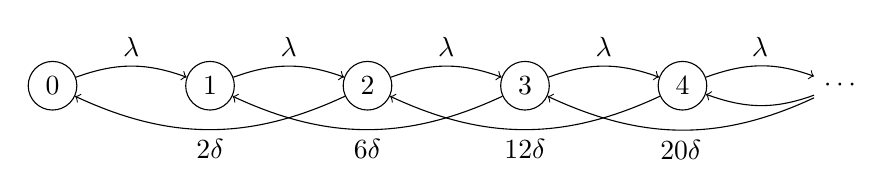
\begin{tikzpicture}{thick}
    \node (n0) at (0, 0) [shape=circle, draw] {$0$};
    \node (n1) at (2, 0) [shape=circle, draw] {$1$};
    \node (n2) at (4, 0) [shape=circle, draw] {$2$};
    \node (n3) at (6, 0) [shape=circle, draw] {$3$};
    \node (n4) at (8, 0) [shape=circle, draw] {$4$};
    \node (n5) at (10, 0) {$\cdots$};

    \draw[->] (n0) edge[out=20, in=-200] node[above] {$\lambda$} (n1);
    \draw[->] (n1) edge[out=20, in=-200] node[above] {$\lambda$} (n2);
    \draw[->] (n2) edge[out=20, in=-200] node[above] {$\lambda$} (n3);
    \draw[->] (n3) edge[out=20, in=-200] node[above] {$\lambda$} (n4);
    \draw[->] (n4) edge[out=20, in=-200] node[above] {$\lambda$} (n5);

    \draw[<-] (n0) edge[out=-25, in=-155] node[below] {$2 \delta$} (n2);
    \draw[<-] (n1) edge[out=-25, in=-155] node[below] {$6 \delta$} (n3);
    \draw[<-] (n2) edge[out=-25, in=-155] node[below] {$12\delta$} (n4);
    \draw[<-] (n3) edge[out=-25, in=-155] node[below] {$20\delta$} (n5);
    \draw[<-] (n4) edge[out=-20, in=-160] (n5);
\end{tikzpicture}
\end{figure}

For a state $(x^{(M)}, x^{(D)})\in\mathbb{N}^2$, where $x^{(M)}\geq 2$,
the \ac{CME} \eqref{eq:cme} becomes
\begin{align*}
    & \frac{d}{dt}\pi((x^{(M)}, x^{(D)}), t)\\
    = \;\,&  \frac{\delta}{2} \, (x^{(M)}+2) (x^{(M)} + 1) \pi((x^{(M)}+2, x^{(D)}-1), t)\\
    & - (\lambda + \frac{\delta}{2} \, x^{(M)} (x^{(M)} - 1))\pi((x^{(M)}, x^{(D)}), t)\\
    & + \lambda \pi((x^{(M)}-1, x^{(D)}), t)
\end{align*}
\end{example}

The explicit representation of all state probabilities is often not possible, because
there are infinitely many states. Usually the state-space is truncated to contain all
relevant states~\parencite{andreychenko2011parameter} or one switches to
an approximation such as the mean-field~\parencite{bortolussi2013continuous}


\section{State-Space Truncation}\label{sec:fsp}
A complete solution of \eqref{eq:cme} is usually not possible.
If the state-space with non-negligible probability is suitably small, a state space
truncation can be performed.
That is, \eqref{eq:cme} is integrated on a possibly time-dependent subset
$\hat{\mathcal{S}}_t\subseteq\mathcal{S}$ \parencite{henzinger2009sliding,munsky2006finite,spieler2014numerical}.
Transitions to states, that are not part of this subset are typically re-directed to a introduced sink-state.
This state captures the mass ``lost'' by the approximation and gives the error up to the numerical integration scheme.\marginpar{Uniformization can give a lower bound on the error.}
\citet{munsky2006finite} coined the term of \acf{FSP} for such a method.

To analyze the stationary distribution (\autoref{sec:stationary_dist}) the redirection scheme needs to be altered \parencite{kuntz2021stationary}:
Instead of a re-redirection into a sink-state, transitions are redirected in \emph{some fashion} back into the truncation set.

\begin{example} Consider a birth-death process as a simple example. This model is used to describe a wide variety of phenomena and often constitutes a sub-module of larger models.
For example, it represents an M/M/1 queue with service rates being linearly dependent on the queue length.
Note that even for this simple model, the state-space is countably infinite.
    \marginpar{This process occurs in many different varieties. For example, the state-space may be finite and propensities are non-polynomial \parencite[see][]{backenkohler2020birth}.}
% \MB{could remove model environment for space}
\begin{model}[Birth-Death Process]\label{model:bd}
The model consists of exponentially distributed arrivals and service times proportional to queue length. It can be expressed using two mass-action reactions:
    \[ \varnothing \xrightarrow{\mu} S \qquad\text{and}\qquad S \xrightarrow{\gamma} \varnothing\,.\]
The initial condition $X_0=0$ holds with probability one.
\end{model}
    The underlying \ac{CTMC} has the following infinite structure.
\vspace{2em}\\
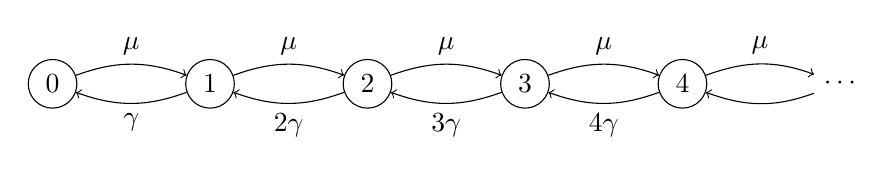
\begin{tikzpicture}{thick}
    \node (n0) at (0, 0) [shape=circle, draw] {$0$};
    \node (n1) at (2, 0) [shape=circle, draw] {$1$};
    \node (n2) at (4, 0) [shape=circle, draw] {$2$};
    \node (n3) at (6, 0) [shape=circle, draw] {$3$};
    \node (n4) at (8, 0) [shape=circle, draw] {$4$};
    \node (n5) at (10, 0) {$\cdots$};

    \draw[->] (n0) edge[out=20, in=-200] node[above] {$\mu$} (n1);
    \draw[->] (n1) edge[out=20, in=-200] node[above] {$\mu$} (n2);
    \draw[->] (n2) edge[out=20, in=-200] node[above] {$\mu$} (n3);
    \draw[->] (n3) edge[out=20, in=-200] node[above] {$\mu$} (n4);
    \draw[->] (n4) edge[out=20, in=-200] node[above] {$\mu$} (n5);

    \draw[<-] (n0) edge[out=-20, in=-160] node[below] {$  \gamma$} (n1);
    \draw[<-] (n1) edge[out=-20, in=-160] node[below] {$2 \gamma$} (n2);
    \draw[<-] (n2) edge[out=-20, in=-160] node[below] {$3 \gamma$} (n3);
    \draw[<-] (n3) edge[out=-20, in=-160] node[below] {$4 \gamma$} (n4);
    \draw[<-] (n4) edge[out=-20, in=-160] (n5);
\end{tikzpicture}
\vspace{2em}\\
The change of probability mass in a single state $x>0$ is described by expanding
\eqref{eq:cme} and
\begin{multline}\label{eq:cme_bd}
    \frac{d}{dt}\pi_t(x)=\mu \pi(x-1, t) + \gamma (x+1) \pi(x+1, t)\\
    - (\mu + \gamma x)\pi(x, t)\,.
\end{multline}
A typical truncation scheme to $[0, N]$ would use \eqref{eq:cme_bd} for $x\in[0,\dotsc,N - 1]$
and for $x=N$ the transition to $N+1$ via the first reaction is re-directed into a sink state.
    We can drop the sink state because of the invariant $\sum_{x}\pi_t(x) = 1$, $\forall t\geq 0$.\marginpar{In general, we can drop one equation in the \ac{CME} system because of this invariant.}
    The \ac{ODE} for the boundary state would consequently read
\[
    \frac{d}{dt}\pi_t(N)=\mu \pi(N-1, t) - (\gamma N + \mu)\pi(N, t)\,.
\]
    Visualizing the resulting \ac{CTMC} and letting $N=3$.
\vspace{2em}\\
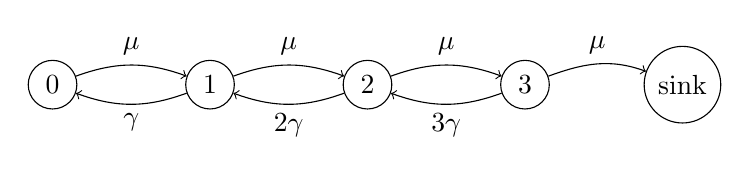
\begin{tikzpicture}{thick}
    \node (n0) at (0, 0) [shape=circle, draw] {$0$};
    \node (n1) at (2, 0) [shape=circle, draw] {$1$};
    \node (n2) at (4, 0) [shape=circle, draw] {$2$};
    \node (n3) at (6, 0) [shape=circle, draw] {$3$};
    \node (n4) at (8, 0) [shape=circle, draw] {sink};

    \draw[->] (n0) edge[out=20, in=-200] node[above] {$\mu$} (n1);
    \draw[->] (n1) edge[out=20, in=-200] node[above] {$\mu$} (n2);
    \draw[->] (n2) edge[out=20, in=-200] node[above] {$\mu$} (n3);
    \draw[->] (n3) edge[out=20, in=-200] node[above] {$\mu$} (n4);

    \draw[<-] (n0) edge[out=-20, in=-160] node[below] {$  \gamma$} (n1);
    \draw[<-] (n1) edge[out=-20, in=-160] node[below] {$2 \gamma$} (n2);
    \draw[<-] (n2) edge[out=-20, in=-160] node[below] {$3 \gamma$} (n3);
\end{tikzpicture}
\vspace{2em}\\
In a forward analysis, the sink state accumulates mass ``lost'' by the approximation.
    This provides a good practical error bound\marginpar{The accuracy of the bound is dependent on the specific method of the forward analysis. Numerical integration, for example, it is less strict.}
    for the chosen truncation.

If one is interested in the stationary probability distribution (\autoref{sec:stationary_dist}), a sink state is not practical, since --~in the long run~-- the process will usually enter such a state.
Instead, the cut transitions are re-directed back into the truncation.
A plethora of re-directions is possible \parencite{gupta2017finite,kuntz2021stationary,spieler2014numerical}, but in general it is reasonable to re-direct to states with cut incoming transitions.\marginpar{Such re-directions are used in \autoref{ch:statagg}.}
In this example, this is equivalent to cutting the transition, because the truncation has only this border state.
\vspace{2em}\\
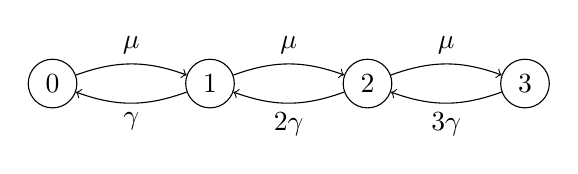
\begin{tikzpicture}{thick}
    \node (n0) at (0, 0) [shape=circle, draw] {$0$};
    \node (n1) at (2, 0) [shape=circle, draw] {$1$};
    \node (n2) at (4, 0) [shape=circle, draw] {$2$};
    \node (n3) at (6, 0) [shape=circle, draw] {$3$};

    \draw[->] (n0) edge[out=20, in=-200] node[above] {$\mu$} (n1);
    \draw[->] (n1) edge[out=20, in=-200] node[above] {$\mu$} (n2);
    \draw[->] (n2) edge[out=20, in=-200] node[above] {$\mu$} (n3);

    \draw[<-] (n0) edge[out=-20, in=-160] node[below] {$  \gamma$} (n1);
    \draw[<-] (n1) edge[out=-20, in=-160] node[below] {$2 \gamma$} (n2);
    \draw[<-] (n2) edge[out=-20, in=-160] node[below] {$3 \gamma$} (n3);
\end{tikzpicture}
\vspace{2em}\\
Thus, the \ac{ODE} for state $N$ here reads
\[
    \frac{d}{dt}\pi_t(N)=\mu \pi(N-1, t) - \gamma N\pi(N, t)\,.
\]
\end{example}

\section{Stochastic Simulations}\label{sec:ssa}
We can generate trajectories of this model using the \acf{SSA} (\autoref{alg:ssa})  \parencite{gillespie1977exact}.
The simulation algorithm consists of repeatedly evaluating the race condition and jump times induced by~\eqref{eq:cme_generator} until some terminal criterion such as a maximum simulation time $T$ is reached (\autoref{line:loop}).
In particular, the algorithm iteratively chooses a reaction, with a probability that is
proportional to its rate given the current state $s$ (\autoref{line:sample_r}).
The jump time $t_j- t_{j+1}$ is determined by sampling from an exponential distribution with rate $\sum_i\alpha_i(s)$ (\autoref{line:sample_dt}).
\begin{algorithm}
\SetKwInOut{Input}{input}
\SetKwInOut{Output}{output}
    \Input{$\pi_0, A$}
    \Output{trajectory $\tau$}
    $\tau \leftarrow$ empty list, $s\leftarrow$ sample from $\pi_0$, $t\leftarrow 0$\;
    \While{$t<T$\label{line:loop}}{
    $\tau\leftarrow \text{append}(\tau, (s, t))$\;
        $k\leftarrow$ sample reaction $i$ with probability $\alpha_i(s)/\sum_i\alpha_i(s)$\label{line:sample_r}\;
    $\delta\sim \text{Exp}\left(\sum_i \alpha_i(s)\right)$\label{line:sample_dt}\;
        $s\leftarrow s + v_k$\;
    $t \leftarrow t + \delta$\;
    }
    \textbf{return} $\tau$\;
    \caption{\label{alg:ssa}Sample a trajectory}
\end{algorithm}

The output of \autoref{alg:ssa} is an alternating sequence of states and jump times
\[
    \tau = s_0t_0s_1t_1\dots t_n s_n, \quad t\in[0,T]
\]
called a \emph{trajectory}.

Monte Carlo estimation requires a sufficiently large number of such trajectories to
be generated.
This collection of realizations facilitates a statistical estimate of
a wide range of quantities such as expected values and probabilities.
The main benefit of this approach is its flexibility.
It can solve essentially all relevant tasks.
The main drawback is the cost associated with the generation of a sufficiently large trajectory ensemble.
This problem becomes very pronounced in case of rare event probability estimation and stiff systems.
\marginpar{Bespoke techniques for these scenarios are available \parencite{cao2005slow,daigle2011automated}.}
Furthermore, the results only provide --~by their very nature~-- statistical guarantees.
Other methods such as explicit state-space representations can give stronger guarantees.


\section{Moment Dynamics}\label{sec:moments_bg}
Often times, the moments of a stochastic process provide sufficient information for its analysis.
%Such is the case for the \emph{mean-field} analysis, where only the expectations \parencite{bortolussi2020fluid}
% are considered, while covariances are assumed to be zero.
\acp{ODE} for the expected values of an \ac{MPM} can be derived using its generator.
We can apply $Q$ to a polynomial $f$ such that\marginpar{This is called the \emph{drift} (see \autoref{sec:statagg:lyapunov}).}
\begin{equation}\label{eq:Qf}
    Qf(x) = \sum_{j=1}^{n_R}\left(f(x+v_j) - f(x)\right)\alpha_j(x)\,.
\end{equation}
By definition of the generator \eqref{eq:generator}
\[
    \frac{d}{dt}\E{f(X_t)|X_t=x} = Qf(x)\,.
\]
Left-multiplying the probability of a given state and summing up over all states, we
obtain the time derivative of the expected value $\expSym(f(X_t))$.
Written as a matrix vector product
\[
    \frac{d}{dt}(\pi f) = \pi Qf\,.
\]
For \acp{MPM}, in particular, we arrive at the functional form
\begin{equation}\label{eq:mom_ode}
    \frac{d}{dt}\E{f({\vec{ X}}_t)} = \sum_{j=1}^{n_R}\E{\left(f({\vec X_t +
    \vec{v}_j}) - f(\vec X_t)\right)\alpha_j(\vec X_t)}\,.
\end{equation}
This equation is used to analyse (raw) \emph{moments} of the process.
\graffito{\emph{Centered} moments (e.g.\ variance) are equivalent via the binomial transform.}
A raw moment is
\[\E{\vec X^{\vec m}}=\E{\prod_{i=1}^{n_S} X_i^{m_i}}\,,\quad \vec m\in {\mathbb{N}}^{n_S}\]
with respect to some probability measure.
An \ac{ODE} is given by \eqref{eq:mom_ode}, setting $f(x)=x^m$.
The \emph{order} of a moment $E({\vec X}^{\vec m})$ is given by the sum of its exponents,
i.e.\ $\sum_i m_i$.
Note that the notion of  expected value can be generalized
to any measure $\mu$ on a Borel-measurable space
$(E, \mathcal{B}(E))$, where
 the $\vec{m}$-th raw moment is $\int_E {\vec x}^{\vec m}\,d\mu(\vec x)$.
Throughout we assume that moments of arbitrary order remain finite over time,
i.e.\ $E(\lvert \vec{X}^{\vec{m}}_t\rvert)<\infty$, $t\geq 0$.
In \citet{gupta2014scalable} the authors propose a framework to verify
this property for a given model.

\begin{example} Let us express the dynamics of the first two uncentered moments for \autoref{model:bd} using \eqref{eq:mom_ode}.
\begin{equation}\label{eq:bd:mom1}
    \begin{split}
    \frac{d}{dt}\E{X_t} =\; &\mu - \gamma \E{X_t}\\
    \frac{d}{dt}\E{X_t^2} =\; &\mu(2\E{X_t} + 1) - \gamma (2\E{X_t^2}-\E{X_t})%     −2𝑑𝑥2+𝑑𝑥+2𝑔𝑥+𝑔
    \end{split}
\end{equation}
Setting initial moments these equations give as an \ac{IVP}, we can solve (see \autoref{fig:momsandprobs}).
This, however, is more an exception than the norm:
Unless all ractions have linear or constant rate functions $\alpha_i(\cdot)$, $\forall i$, we would not end up with a closed system of \acp{ODE} as in \eqref{eq:bd:mom1}.
To illustrate, let us pretend the reaction ($S\xrightarrow{\gamma}\varnothing$) would become this non-linear reaction\graffito{The model is then the same as \autoref{model:dim}.}
    \[
2S\xrightarrow{\gamma}\varnothing\,.
\]
Accordingly, due to mass-action \eqref{eq:stoch_mass_action}
    \[
\alpha_2(x)=\gamma (x^2 - x)\,.
\]
Therefore the first moment's derivative becomes
    \[
\frac{d}{dt}\E{X_t} =\mu - \gamma \left(\E{X_t^2} - \E{X_t}\right)\,.
\]
Note, that now the right-hand side of the derivative in the example depends on the value of the second moment $\E{X_t^2}$.
\end{example}
If we consider the general expression \eqref{eq:mom_ode} for the moment of order $k$ clearly a term of order $k+1$ occurs, that does (usually) not cancel out if a propensity function is at least
quadratic.
Therefore, researches commonly rely on ad-hoc approximations to truncate this infinite system of \acp{ODE} \parencite{hespanha2008moment,schnoerr2015,schnoerr2014validity}.
Unfortunately such schemes have typically no guarantees to converge --~or even improve~-- with increasing truncation order \parencite{schnoerr2014validity} or increasing system size.
Furthermore,
\marginpar{This finite moment problem could also be posed as a \acl{GMP}\@. The resulting \ac{SDP} can be solved numerically \parencite{lasserre2010moments}.}
fairly involved numerical schemes have to be employed to recover distributional approximations \parencite{andreychenko2017distribution}.
The only scheme with a convergence guarantee in the system size limit is the \emph{mean-field} approximation \parencite{bortolussi2013continuous}.
Therein zero-covariances are assumed, i.e.\ the system is truncated at the first oder equations using the approximation $\E{X_t^2}=\E{X_t}^2$.
\begin{figure}[htb]
    \centering
    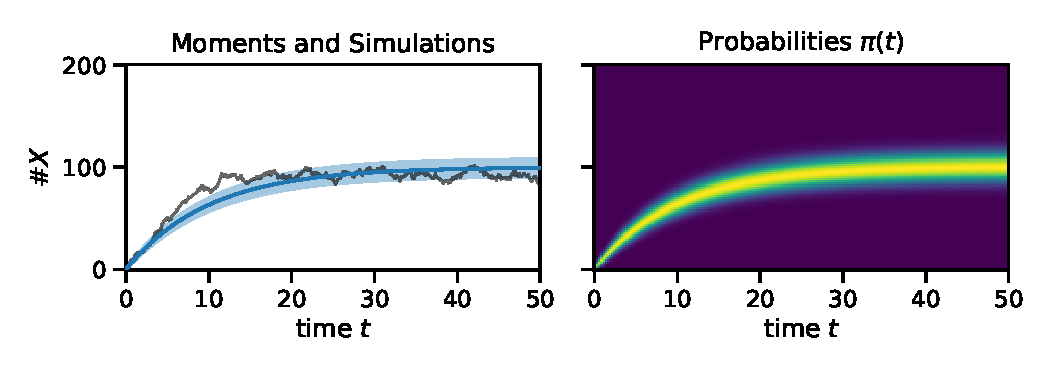
\includegraphics[width=0.9\textwidth]{gfx/momsandprobs.pdf}
    \caption[Moments and probability distribution $\pi(t)$]{\label{fig:momsandprobs}The expected value $\pm$ a standard deviation along with a sampled trajectory (left) and the probability distribution over time (right) of \autoref{model:bd} with $\mu=10$ and $\gamma=0.1$.}
\end{figure}

\subsection{Hybrid Representations}
Especially in biological applications ithe abundancies of individual species vary by orders
of magnitude within one model.
A canonical example of this fact are classic gene expression models, where proteins are expressed
conditional on a binary gene state.
To approximate such variables using a moment approximation, or even mean-field, does not make too much sense since such approximations either hinge on the high abundancy of the species or try to alleviate state-space explosion stemming from it.
Hybrid methods leverage the best of both worlds by approximating larger populations using continuous approximations such as moment closures, while small popuations are modeled discretely.

An example of such an approach is the \ac{MCM} presented in \citet{hasenauer2014method} and \citet{kazeroonian2014modeling}.
In this approach species are split into a high-count component $\tilde{X}_t$ and a low-count component $\hat{X}_t$.
Then the partial expectations
\begin{equation}\label{eq:cm}
    \E{\tilde{X}_t \mid \hat{X}_t = \hat{x}}\Pr({\hat{X}_t=\hat{x}})
\end{equation}
are approximated for all or some valuations $\hat{x}$ using a standard moment closure \parencite{andreychenko2015reconstruction}.
Equivalent results for \eqref{eq:cm} can be achieved by using that $\E{\hat{X}}=\E{\hat{X}^m}$, $m\geq 1$ for a Bernoulli random variable.

%Equivalent results are obtained by modifying the network to have 1 species per abundancy (basically rule based)
%\parencite{hasenauer2014method,kazeroonian2014modeling,andreychenko2015reconstruction}

\section{Stationary Distribution}\label{sec:stationary_dist}
Assuming
% irreducibility and
ergodicity
of the underlying chain, a stationary distribution $\pi_{\infty}$ is an invariant distribution, namely a fixed point of the Kolmogorov forward equation \eqref{eq:forward}.
Let $\pi_{\infty}$ be the vector description of a stationary distribution. It then  satisfies
\begin{equation}\label{eq:stationary}
0=\pi_{\infty}Q\quad
\end{equation}
as a fixed point of the Kolmogorov equation \eqref{eq:forward}.
Furthermore, the solution is constrained, to form a probability distribution, i.e.\ a measure with
unit mass. Thus,
\begin{equation}
1=\sum_{x\in\mathcal{S}}\pi_{\infty}(x)\,.
\end{equation}
Stationary distributions are connected to the \emph{long-run} behavior of an \ac{MPM}~\parencite{dayar2011bounding}, as the system's distribution will converge to the (unique)
stationary distribution.
The connection of the stationary distribution to the long-run behavior becomes clear when considering the ergodic theorem.
For some $A\subseteq\mathcal{S}$,
\begin{equation}\label{eq:ergodic}
    \lim_{T\to\infty}\frac{1}{T}\int_0^T 1_A(X_t)\,dt
    = \sum_{x\in A}\pi_{\infty}(x)\,.
\end{equation}
Thus, the mean occupation time for set $A$ over infinite trajectories is the stationary measure for $A$.
Eq.~\eqref{eq:ergodic} shows that we can assess long-run behavior using the stationary distribution and vice-versa.

\begin{example}
    Returning to the example of \autoref{model:bd} it is obvious that the state-space is irreducible.
Further, we can easily show, that the stationary distribution is Poissonian with rate $\mu/\gamma$:
    \[ \pi_{\infty}(x)=\frac{{(\mu/\gamma)}^{x}\exp(-\mu/\gamma)}{x!}\,.\]
\end{example}


For simplicity, we assume throughout that the state-space is composed of a single communicating class.
Checking ergodicity given a countably infinite number of states is achieved by providing a suitable Foster-Lyapunov function \parencite{meyn2012markov}.
Some automated techniques have been proposed for this task \parencite{dayar2011bounding,gupta2014scalable,milias2014optimization}.



\subsection{Foster-Lyapunov Bounds}\label{sec:statagg:lyapunov}
It is well-known that for a \ac{CTMC} $X$, ergodicity can be proven by a Foster-Lyapunov
 function $g:\mathcal{S}\to\mathbb{R}$ \parencite{meyn1993stability,dayar2011bounding}.
 This is the stochastic analogue of the Lyapunov functions, used to prove convergence of \acp{ODE}\@.
%The positivity requirement can somewhat be relaxed. The function only needs to be bounded from below since it can be shifted to the positives. In practice this shift can be ignored since it cancels out in the drift \eqref{eq:drift}.
The function $g$ is required to have finite level sets:
\[
    \left|\{x\in\mathcal{S} \mid g(x) < l\}\right|<\infty,\quad \forall l > 0.
\]
Typical choices for $g$ are linear \parencite{gupta2014scalable,milias2014optimization} or quadratic \parencite{spieler2014numerical}.
Given the $g$, we define its \emph{drift} $d$ as its average infinitesimal change, which is obtained applying the generator $Q$ to $g$.\marginpar{Intuitively, $g$ is interpreted as a vector with the values $f(x_i)_i=f_i$ with the same ordering as in $Q$.}% See also \autoref{sec:moments_bg}.}
\begin{equation}\label{eq:drift}
    d(x) = Qg(x) = \sum_{j=1}^{n_R} \alpha_j(x) (g(x+v_j) -  g(x))
\end{equation}
As such the drift can be interpreted as the expected local tendency of change of a scalar valued function $g$, \marginpar{Note that we end up with \eqref{eq:mom_ode} taking the expectation.}i.e.\
\[
    d(x) = \frac{d}{dt}\E{g(X_t)\mid X_t = x}\,.
\]
A Lyapunov function can be used to prove ergodicity of a \ac{CTMC}: If there is a finite subset $C\subset\mathcal{S}$ such that
\begin{align}
    &Qg(x)\leq -1,\; \forall x\in\mathcal{S}\setminus C\,,\label{eq:neg_outside}\\
    &Qg(x)< \infty,\; \forall x\in C\,, \text{ and}\label{eq:pos_inside}\\
    &\lVert x\rVert\to\infty \Rightarrow g(x)\to\infty\,,\;\text{ where }\;\lVert x\rVert=\sum_i x_i\,,\label{eq:lya_normlike}
\end{align}
then the chain is non-explosive and ergodic~\parencite{milias2014optimization,tweedie_1975}.
Intuitively, $g(X_t)$ should be a supermartingale outside $C$ and a submartingale inside.
Since the $g$ is norm-like due to \eqref{eq:lya_normlike} this entails that the process
tends towards $C$ when outside, and out of from $C$ when inside.


Given the above requirements
\begin{equation}\label{eq:lyapunov_set}
    \mathcal{C}_{\epsilon_{\ell}} = \left\{ x\in\mathcal{S} \mid
    \frac{\epsilon_{\ell}}{c}d(x) > \epsilon_{\ell} - 1\right\}
\end{equation}
is finite, where
\[
    \infty> c\geq \sup_{x\in\mathcal{S}} d(x)\,.
\]
In this case, $\mathcal{C}_{\epsilon_{\ell}}$ contains at least $1-\epsilon_{\ell}$ of stationary probability mass for any $\epsilon_{\ell}\in(0,1)$ \parencite[][Thm.~8]{spieler2014numerical}.
Given that $\mathcal{C}_{\epsilon_{\ell}}$ is finite, the chain is ergodic and
\begin{equation}
    \sum_{x\in\mathcal{C}_{\epsilon_{\ell}}}\pi(x)> 1 - \epsilon_{\ell}
\end{equation}
bounding the stationary probability mass contained within $\mathcal{C}_{\epsilon_{\ell}}$.
\begin{example}
    We return to \autoref{model:bd} and choose $g(x) = x$.
    Then \[ d(x) = \mu - \gamma x\,. \]
    The requirements \eqref{eq:neg_outside}, \eqref{eq:pos_inside},
    and \eqref{eq:lya_normlike} are fulfilled for
    \[ C=\left\{0,\dotsc,\frac{1+\mu}{\gamma} - 1\right\} \]
    and the underlying chain is ergodic. We can further bound the stationary distribution.
    Letting $c=\mu$,
    \[ \frac{\epsilon_{\ell}}{\mu}d(x) = \epsilon_{\ell} - \frac{\epsilon_{\ell}\gamma}{\mu}x \]
    and following \eqref{eq:lyapunov_set} the states
    \[ 0\leq x<\frac{\mu}{\epsilon_{\ell}\gamma}  \]
    have at least $1-\epsilon_{\ell}$ stationary mass.
\end{example}



\section{A Brief Taxonomy of Multimodality}\label{sec:multimodality}
Multimodality is an overloaded term in the context of reaction network models.
Specifically, it can be used to describe the following features.
\begin{description}
    \item[Operational Multimodality]
        This kind of multimodality characterizes the model behavior directly.
        Consider, for example, a gene
        expression model\marginpar{See \autoref{model:gexpr}
        on page~\pageref{model:gexpr} for an example of this.}:
        The gene state is digital, meaning it is either active or inactive.
        Depending on this state a protein is either synthesized or not.
        Therefore the system has distinct \emph{operational modes}
        which dictate its dynamics.
        Non-biological examples can be found in the
        context of broadcasting systems,
        in which the dynamics change discretely due to messages shared between
        agents~\parencite{bortolussi2020fluid}.

        Naturally, nearly all models change their dynamics,
        given a change in their state vector.
        In this aspect this distinction is not wholly strict.
        It is mainly intended to indicate distinctive changes in the dynamics.
        In some instances, these can be as obvious as the examples mentioned above.
        In other cases they may not be as obvious:
        Consider an epidemics die-out for example, which is a significant change
        in the operating mode, which is not due to a switch-type reaction.
  \item[Distributional Multimodality]
        This kind of multimodality is characterized by the stationary distribution $\pi_{\infty}$:
        It has multiple
        \emph{modes}, i.e.\ local maxima. Given an ergodic underlying \ac{CTMC}
        this entails, that the system spends most time in distinct regions of the
        state-space (cf.\ \eqref{eq:ergodic}).
        The \emph{switching} between those distinct region is of interest
        for both, analysis and control, of such models.
\end{description}
While distributional multimodality implies operational multimodality, the reverse
does not hold.

% Literature:
% \begin{itemize}
%     \item \parencite{siegal2011emergence}
% \end{itemize}
